%No intervention graph actualization

% tikzpic.teP
\documentclass[crop,tikz]{standalone}% 'crop' is the default for v1.0, before it was 'preview'

%Packages
\usepackage{xcolor}

%tikz libraries}}
\usetikzlibrary{shapes.geometric,decorations.markings,positioning,calc}

%Colors
\definecolor{susceptible}{RGB}{141,160,203}
\definecolor{recovery}{RGB}{102,194,165}
\definecolor{infection}{RGB}{252,141,98}
% \definecolor{intervention}{RGB}{231,138,195}
\definecolor{intervention}{RGB}{50, 102, 86}
\definecolor{nothing}{RGB}{225,225,225}

%New commands
\newcommand{\Leftscissor}{\large  X}
\newcommand{\Largescissor}{\Huge  X}

\newcommand{\independentedge}[5]{
  % \draw[-latex,potential,line width=1mm, color=#5] (#1) -- (#2);
  \draw[#3, color=#4] (#1) -- ($(#1)!.5!(#2)$);
  \draw[-latex,#3, color=#5] ($(#1)!.5!(#2)$) -- (#2);
  \draw ($(#1)!.5!(#2)$) node[draw=black,fill=#5,#3,line width=.1mm,diamond] {};
}
\newcommand{\contactedge}[9]{
  \pgfmathsetmacro{\s}{1-#7}
  \pgfmathsetmacro{\outangle}{.5*(#8 + #9)};
  \pgfmathsetmacro{\inangle}{180+.5*(#8 + #9)};
  \pgfmathsetmacro{\inangleend}{180+(#9)};
  \pgfmathsetmacro{\eventangle}{\outangle};

  \node (sum) at  ($(#1)!.6!(#3)$) (E121) {};
  \node (sum) at ($(#2)!.6!(#3)$) (E122) {};
  \node (sum) at ($(E121)!\s!(E122)$) (E12) {};
  \draw[-latex,#4,color=#6,tangent=.5] (#1) to[out=#9,in=\inangle] (E12.center) to[out=\outangle,in=\inangleend] (#3);
  \draw (tangent point-1) node (tp1) {};
  \draw (tangent unit vector-1) node (tv1) {};
  \draw (tangent orthogonal unit vector-1) node (to1) {};
  \draw[-,#4,color=#5,tangent=.5] (#2) to[out=#8,in=\inangle] (E12.center);
  \draw (tangent point-1) node (tp2) {};
  \draw (tangent unit vector-1) node (tv2) {};
  \draw (tangent orthogonal unit vector-1) node (to2) {};
  \draw ($(tp1)!.5!(tp2)$) node (tp3) {};
  \draw ($(tv1)!.5!(tv2)$) node (tv3) {};
  \draw ($(tv3.center) - (tp3.center)$) node (tv4) {};
  \newdimen\myxcoord
  \newdimen\myycoord
  \pgfextractx{\myxcoord}{(tv4)};
  \pgfextracty{\myycoord}{(tv4)};
  \pgfmathsetmacro{\diamondangle}{atan2(\myycoord,\myxcoord)};
  \draw (E12.center) node[diamond,#4,line width=.1mm,draw=black,fill=#6,rotate=\diamondangle] {};
}

% Formatting macros:
\tikzstyle{node}=[minimum size= .5in,circle, draw]
\tikzset{intervened node fill/.style  args={#1,#2}{node,potential,circle split part fill={#1,#2}}}

\tikzset{potential/.style={opacity=.7}}
\tikzset{actual/.style={opacity=1}}
\tikzset{impossible/.style={opacity=.2}}
\tikzset{y=-1cm}
\tikzset{x=1cm}

\tikzstyle{edge}=[diamond, draw]
\tikzstyle{intervention}=[fill = intervention]
\tikzstyle{contact}=[fill = infection]
\tikzstyle{recovery}=[fill = recovery]

 \makeatletter
\tikzset{%
  tangent/.style={
    decoration={
      markings,% switch on markings
      mark=
        at position #1
        with
        {
          \coordinate (tangent point-\pgfkeysvalueof{/pgf/decoration/mark info/sequence number}) at (0pt,0pt);
          \coordinate (tangent unit vector-\pgfkeysvalueof{/pgf/decoration/mark info/sequence number}) at (1,0pt);
          \coordinate (tangent orthogonal unit vector-\pgfkeysvalueof{/pgf/decoration/mark info/sequence number}) at (0pt,1);
        }
    },
    postaction=decorate
  },
  use tangent/.style={
    shift=(tangent point-#1),
    x=(tangent unit vector-#1),
    y=(tangent orthogonal unit vector-#1)
  },
  use tangent/.default=1
]}
\makeatother


\makeatletter
%% Modifiecd from stack exchange https://tex.stackexchange.com/questions/55594/tikz-two-colored-circle-split
\tikzset{circle split part fill/.style  args={#1,#2}{%
    alias=tmp@name, % Jake's idea !!
    postaction={%
      insert path={
        \pgfextra{%
          \pgfpointdiff{\pgfpointanchor{\pgf@node@name}{center}}%
          {\pgfpointanchor{\pgf@node@name}{north}}%
          \pgfmathsetmacro\scale{1}
          \pgfmathsetmacro\insiderad{\pgf@y*\scale}
          \fill[#1] (\pgf@node@name.base) ([yshift=-\pgflinewidth]\pgf@node@name.north) arc
          (90:270:\insiderad-\pgflinewidth)--cycle;
          \fill[#2] (\pgf@node@name.base) ([yshift=\pgflinewidth]\pgf@node@name.south)  arc
          (270:450:\insiderad-\pgflinewidth)--cycle;            %  \end{scope}
        }}}}}
 \makeatother  
 
 \makeatletter
%% Modifiecd from stack exchange https://tex.stackexchange.com/questions/55594/tikz-two-colored-circle-split
\tikzset{circle tri split part fill/.style  args={#1,#2,#3}{%
    alias=tmp@name, % Jake's idea !!
    postaction={%
      insert path={
        \pgfextra{%
          \pgfpointdiff{\pgfpointanchor{\pgf@node@name}{center}}%
          {\pgfpointanchor{\pgf@node@name}{north}}%
          \pgfmathsetmacro\scale{1}
          \pgfmathsetmacro\insiderad{\pgf@y*\scale}
          \fill[#1] (\pgf@node@name.base) ([yshift=-\pgflinewidth]\pgf@node@name.north) arc
          (90:210:\insiderad-\pgflinewidth)--(\pgf@node@name.center)--cycle;
          \fill[#2] (\pgf@node@name.base) ([yshift=-\pgflinewidth]\pgf@node@name.north)  arc
          (90:-30:\insiderad-\pgflinewidth)--(\pgf@node@name.center)--cycle; 
          \fill[#3] (\pgf@node@name.base) ([yshift=\pgflinewidth]\pgf@node@name.south)  arc
          (-90:-30:\insiderad-\pgflinewidth)--(\pgf@node@name.center)--cycle; 
          \fill[#3] (\pgf@node@name.base) ([yshift=\pgflinewidth]\pgf@node@name.south)  arc
          (270:210:\insiderad-\pgflinewidth)--(\pgf@node@name.center)--cycle;            %  \end{scope}
        }}}}}
 \makeatother

\begin{document}

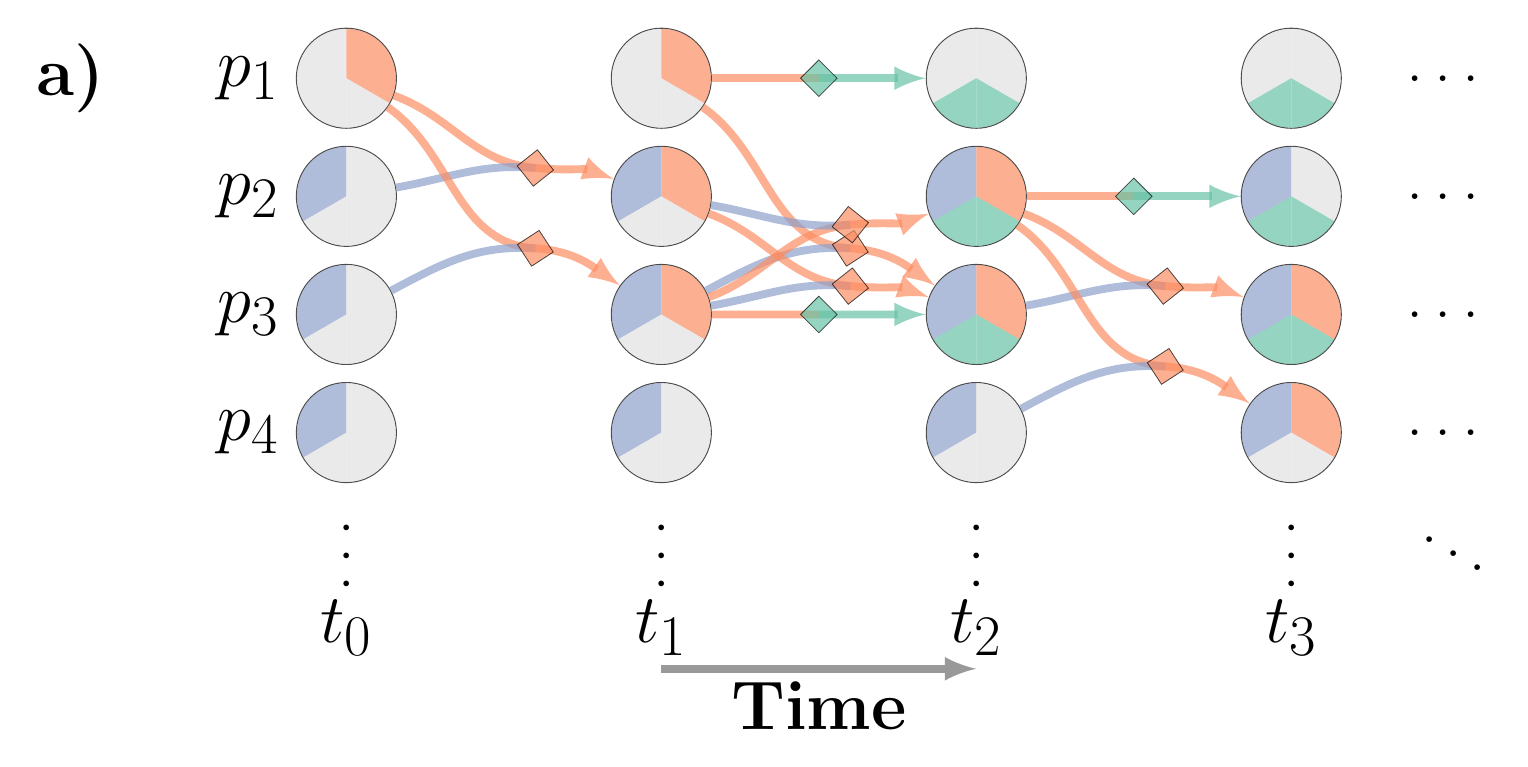
\begin{tikzpicture}
  \draw (-3.5,0) node {\Huge \textbf{a)}};
  \draw (0,0) node[node,potential,circle tri split part fill={nothing,infection,nothing}] (P11) {};
  \draw (0,1.5) node[node,potential,circle tri split part fill={susceptible,nothing,nothing}] (P21) {};
  \draw (0,3) node[node,potential,circle tri split part fill={susceptible,nothing,nothing}] (P31) {};
  \draw (0,4.5) node[node,potential,circle tri split part fill={susceptible,nothing,nothing}] (P41) {};

  \draw (4,0) node[node,potential,circle tri split part fill={nothing,infection,nothing}] (P12) {};
  \draw (4,1.5) node[node,potential,circle tri split part fill={susceptible,infection,nothing}] (P22) {};
  \draw (4,3) node[node,potential,circle tri split part fill={susceptible,infection,nothing}] (P32) {};
  \draw (4,4.5) node[node,potential,circle tri split part fill={susceptible,nothing,nothing}] (P42) {};

  \draw (8,0) node[node,potential,circle tri split part fill={nothing,nothing,recovery}] (P13) {};
  \draw (8,1.5) node[node,potential,circle tri split part fill={susceptible,infection,recovery}] (P23) {};
  \draw (8,3) node[node,potential,circle tri split part fill={susceptible,infection,recovery}] (P33) {};
  \draw (8,4.5) node[node,potential,circle tri split part fill={susceptible,nothing,nothing}] (P43) {};

  \draw (12,0) node[node,potential,circle tri split part fill={nothing,nothing,recovery}] (P14) {};
  \draw (12,1.5) node[node,potential,circle tri split part fill={susceptible,nothing,recovery}] (P24) {};
  \draw (12,3) node[node,potential,circle tri split part fill={susceptible,infection,recovery}] (P34) {};
  \draw (12,4.5) node[node,potential,circle tri split part fill={susceptible,infection,nothing}] (P44) {};

  \contactedge{P11}{P21}{P22}{potential,line width=1mm}{susceptible}{infection}{.6}{10}{-20}
  \contactedge{P11}{P31}{P32}{potential,line width=1mm}{susceptible}{infection}{.7}{28}{-35}
  
  \contactedge{P12}{P32}{P33}{potential,line width=1mm}{susceptible}{infection}{.7}{28}{-35}
  \contactedge{P22}{P32}{P33}{potential,line width=1mm}{susceptible}{infection}{.6}{10}{-20}
  \contactedge{P32}{P22}{P23}{potential,line width=1mm}{susceptible}{infection}{.6}{-10}{20}
 
  \independentedge{P12}{P13}{potential,line width=1mm}{infection}{recovery};
  \independentedge{P32}{P33}{potential,line width=1mm}{infection}{recovery};
  
  \contactedge{P23}{P33}{P34}{potential,line width=1mm}{susceptible}{infection}{.6}{10}{-20}
  \contactedge{P23}{P43}{P44}{potential,line width=1mm}{susceptible}{infection}{.7}{28}{-35}
 
  \independentedge{P23}{P24}{potential,line width=1mm}{infection}{recovery};

  %% Extends on
  \draw (14,0) node{\Huge \dots};
  \draw (14,1.5) node{\Huge \dots};
  \draw (14,3) node{\Huge \dots};
  \draw (14,4.5) node{\Huge \dots};

  \draw (0,6) node[rotate=90]{\Huge \dots};
  \draw (4,6) node[rotate=90]{\Huge \dots};
  \draw (8,6) node[rotate=90]{\Huge \dots};
  \draw (12,6) node[rotate=90]{\Huge \dots};
  \draw (14,6) node[rotate=150]{\Huge \dots};
  %% Legend things
  \draw[-latex,line width=1mm,white!60!black] (4,7.5) -- (8,7.5) node[midway, below,text=black] {\Huge \textbf{Time}};
  \draw (0 ,6.5) node[below,text=black] {\Huge $t_0$};
  \draw (4 ,6.5) node[below,text=black] {\Huge $t_1$};
  \draw (8 ,6.5) node[below,text=black] {\Huge $t_2$};
  \draw (12,6.5) node[below,text=black] {\Huge $t_3$};
  \draw (-1.25,0  ) node[text=black] {\Huge $p_1$};
  \draw (-1.25,1.5) node[text=black] {\Huge $p_2$};
  \draw (-1.25,3  ) node[text=black] {\Huge $p_3$};
  \draw (-1.25,4.5) node[text=black] {\Huge $p_4$};
\end{tikzpicture}

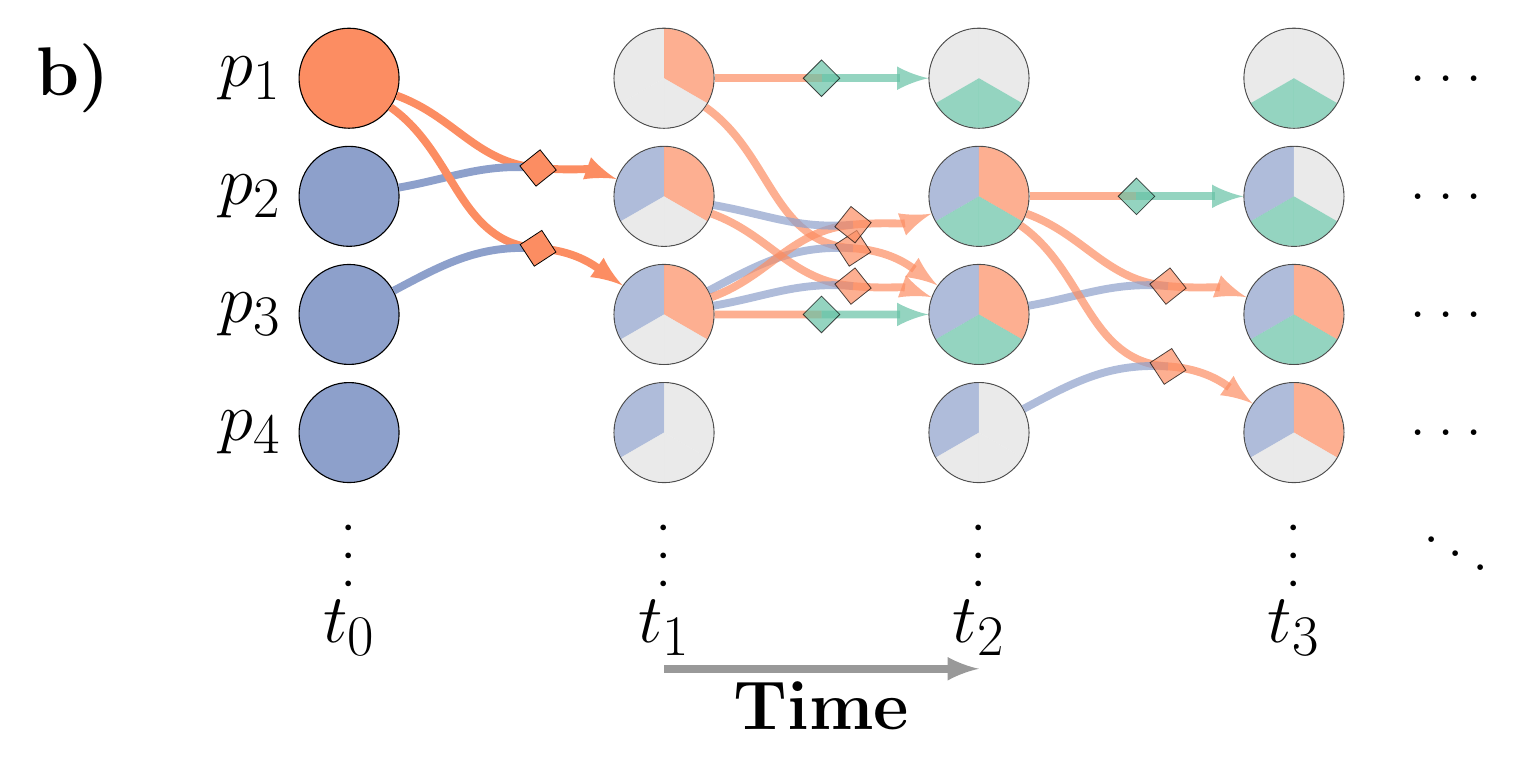
\begin{tikzpicture}
  \draw (-3.5,0) node {\Huge \textbf{b)}};
  \draw (0,0) node[node,actual,circle,fill=infection] (P11) {};
  \draw (0,1.5) node[node,actual,circle,fill=susceptible] (P21) {};
  \draw (0,3) node[node,actual,circle,fill=susceptible] (P31) {};
  \draw (0,4.5) node[node,actual,circle,fill=susceptible] (P41) {};

  \draw (4,0) node[node,potential,circle tri split part fill={nothing,infection,nothing}] (P12) {};
  \draw (4,1.5) node[node,potential,circle tri split part fill={susceptible,infection,nothing}] (P22) {};
  \draw (4,3) node[node,potential,circle tri split part fill={susceptible,infection,nothing}] (P32) {};
  \draw (4,4.5) node[node,potential,circle tri split part fill={susceptible,nothing,nothing}] (P42) {};

  \draw (8,0) node[node,potential,circle tri split part fill={nothing,nothing,recovery}] (P13) {};
  \draw (8,1.5) node[node,potential,circle tri split part fill={susceptible,infection,recovery}] (P23) {};
  \draw (8,3) node[node,potential,circle tri split part fill={susceptible,infection,recovery}] (P33) {};
  \draw (8,4.5) node[node,potential,circle tri split part fill={susceptible,nothing,nothing}] (P43) {};

  \draw (12,0) node[node,potential,circle tri split part fill={nothing,nothing,recovery}] (P14) {};
  \draw (12,1.5) node[node,potential,circle tri split part fill={susceptible,nothing,recovery}] (P24) {};
  \draw (12,3) node[node,potential,circle tri split part fill={susceptible,infection,recovery}] (P34) {};
  \draw (12,4.5) node[node,potential,circle tri split part fill={susceptible,infection,nothing}] (P44) {};

  \contactedge{P11}{P21}{P22}{actual,line width=1mm}{susceptible}{infection}{.6}{10}{-20}
  \contactedge{P11}{P31}{P32}{actual,line width=1mm}{susceptible}{infection}{.7}{28}{-35}
  
  \contactedge{P12}{P32}{P33}{potential,line width=1mm}{susceptible}{infection}{.7}{28}{-35}
  \contactedge{P22}{P32}{P33}{potential,line width=1mm}{susceptible}{infection}{.6}{10}{-20}
  \contactedge{P32}{P22}{P23}{potential,line width=1mm}{susceptible}{infection}{.6}{-10}{20}
 
  \independentedge{P12}{P13}{potential,line width=1mm}{infection}{recovery};
  \independentedge{P32}{P33}{potential,line width=1mm}{infection}{recovery};
  
  \contactedge{P23}{P33}{P34}{potential,line width=1mm}{susceptible}{infection}{.6}{10}{-20}
  \contactedge{P23}{P43}{P44}{potential,line width=1mm}{susceptible}{infection}{.7}{28}{-35}
 
  \independentedge{P23}{P24}{potential,line width=1mm}{infection}{recovery};
 
  %% Extends on
  \draw (14,0) node{\Huge \dots};
  \draw (14,1.5) node{\Huge \dots};
  \draw (14,3) node{\Huge \dots};
  \draw (14,4.5) node{\Huge \dots};

  \draw (0,6) node[rotate=90]{\Huge \dots};
  \draw (4,6) node[rotate=90]{\Huge \dots};
  \draw (8,6) node[rotate=90]{\Huge \dots};
  \draw (12,6) node[rotate=90]{\Huge \dots};
  \draw (14,6) node[rotate=150]{\Huge \dots};
  %% Legend things
  \draw[-latex,line width=1mm,white!60!black] (4,7.5) -- (8,7.5) node[midway, below,text=black] {\Huge \textbf{Time}};
  \draw (0 ,6.5) node[below,text=black] {\Huge $t_0$};
  \draw (4 ,6.5) node[below,text=black] {\Huge $t_1$};
  \draw (8 ,6.5) node[below,text=black] {\Huge $t_2$};
  \draw (12,6.5) node[below,text=black] {\Huge $t_3$};
  \draw (-1.25,0  ) node[text=black] {\Huge $p_1$};
  \draw (-1.25,1.5) node[text=black] {\Huge $p_2$};
  \draw (-1.25,3  ) node[text=black] {\Huge $p_3$};
  \draw (-1.25,4.5) node[text=black] {\Huge $p_4$};
\end{tikzpicture}

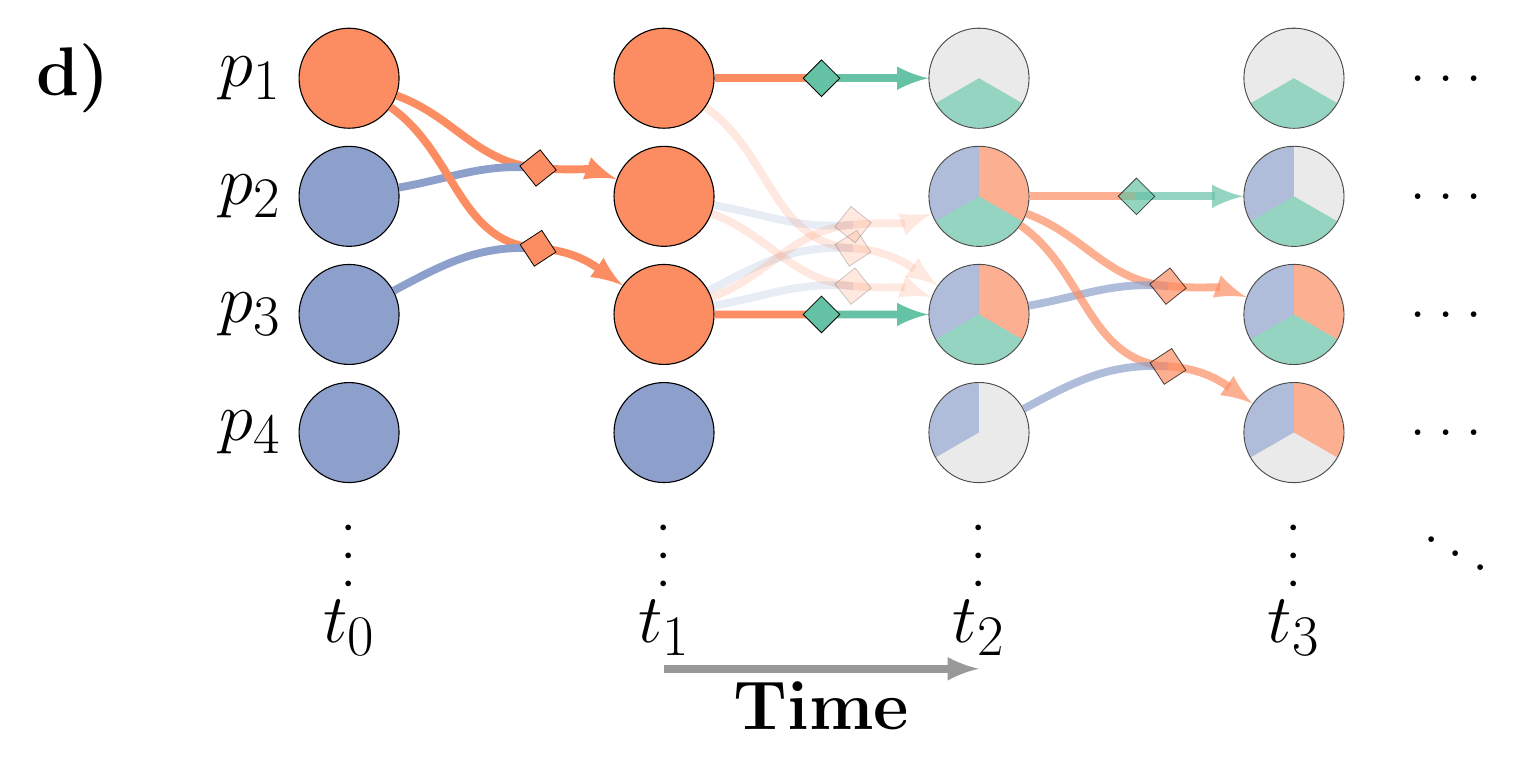
\begin{tikzpicture}
  \draw (-3.5,0) node {\Huge \textbf{d)}};
  \draw (0,0) node[node,actual,circle,fill=infection] (P11) {};
  \draw (0,1.5) node[node,actual,circle,fill=susceptible] (P21) {};
  \draw (0,3) node[node,actual,circle,fill=susceptible] (P31) {};
  \draw (0,4.5) node[node,actual,circle,fill=susceptible] (P41) {};

  \draw (4,0) node[node,actual,circle,fill=infection] (P12) {};
  \draw (4,1.5) node[node,actual,circle,fill=infection] (P22) {};
  \draw (4,3) node[node,actual,circle,fill=infection] (P32) {};
  \draw (4,4.5) node[node,actual,circle,fill=susceptible] (P42) {};

  \draw (8,0) node[node,potential,circle tri split part fill={nothing,nothing,recovery}] (P13) {};
  \draw (8,1.5) node[node,potential,circle tri split part fill={susceptible,infection,recovery}] (P23) {};
  \draw (8,3) node[node,potential,circle tri split part fill={susceptible,infection,recovery}] (P33) {};
  \draw (8,4.5) node[node,potential,circle tri split part fill={susceptible,nothing,nothing}] (P43) {};

  \draw (12,0) node[node,potential,circle tri split part fill={nothing,nothing,recovery}] (P14) {};
  \draw (12,1.5) node[node,potential,circle tri split part fill={susceptible,nothing,recovery}] (P24) {};
  \draw (12,3) node[node,potential,circle tri split part fill={susceptible,infection,recovery}] (P34) {};
  \draw (12,4.5) node[node,potential,circle tri split part fill={susceptible,infection,nothing}] (P44) {};

  \contactedge{P11}{P21}{P22}{actual,line width=1mm}{susceptible}{infection}{.6}{10}{-20}
  \contactedge{P11}{P31}{P32}{actual,line width=1mm}{susceptible}{infection}{.7}{28}{-35}
  
  \contactedge{P12}{P32}{P33}{impossible,line width=1mm}{susceptible}{infection}{.7}{28}{-35}
  \contactedge{P22}{P32}{P33}{impossible,line width=1mm}{susceptible}{infection}{.6}{10}{-20}
  \contactedge{P32}{P22}{P23}{impossible,line width=1mm}{susceptible}{infection}{.6}{-10}{20}
 
  \independentedge{P12}{P13}{actual,line width=1mm}{infection}{recovery};
  \independentedge{P32}{P33}{actual,line width=1mm}{infection}{recovery};
  
  \contactedge{P23}{P33}{P34}{potential,line width=1mm}{susceptible}{infection}{.6}{10}{-20}
  \contactedge{P23}{P43}{P44}{potential,line width=1mm}{susceptible}{infection}{.7}{28}{-35}
 
  \independentedge{P23}{P24}{potential,line width=1mm}{infection}{recovery};

  %% Extends on
  \draw (14,0) node{\Huge \dots};
  \draw (14,1.5) node{\Huge \dots};
  \draw (14,3) node{\Huge \dots};
  \draw (14,4.5) node{\Huge \dots};

  \draw (0,6) node[rotate=90]{\Huge \dots};
  \draw (4,6) node[rotate=90]{\Huge \dots};
  \draw (8,6) node[rotate=90]{\Huge \dots};
  \draw (12,6) node[rotate=90]{\Huge \dots};
  \draw (14,6) node[rotate=150]{\Huge \dots};
  %% Legend things
  \draw[-latex,line width=1mm,white!60!black] (4,7.5) -- (8,7.5) node[midway, below,text=black] {\Huge \textbf{Time}};
  \draw (0 ,6.5) node[below,text=black] {\Huge $t_0$};
  \draw (4 ,6.5) node[below,text=black] {\Huge $t_1$};
  \draw (8 ,6.5) node[below,text=black] {\Huge $t_2$};
  \draw (12,6.5) node[below,text=black] {\Huge $t_3$};
  \draw (-1.25,0  ) node[text=black] {\Huge $p_1$};
  \draw (-1.25,1.5) node[text=black] {\Huge $p_2$};
  \draw (-1.25,3  ) node[text=black] {\Huge $p_3$};
  \draw (-1.25,4.5) node[text=black] {\Huge $p_4$};
\end{tikzpicture}

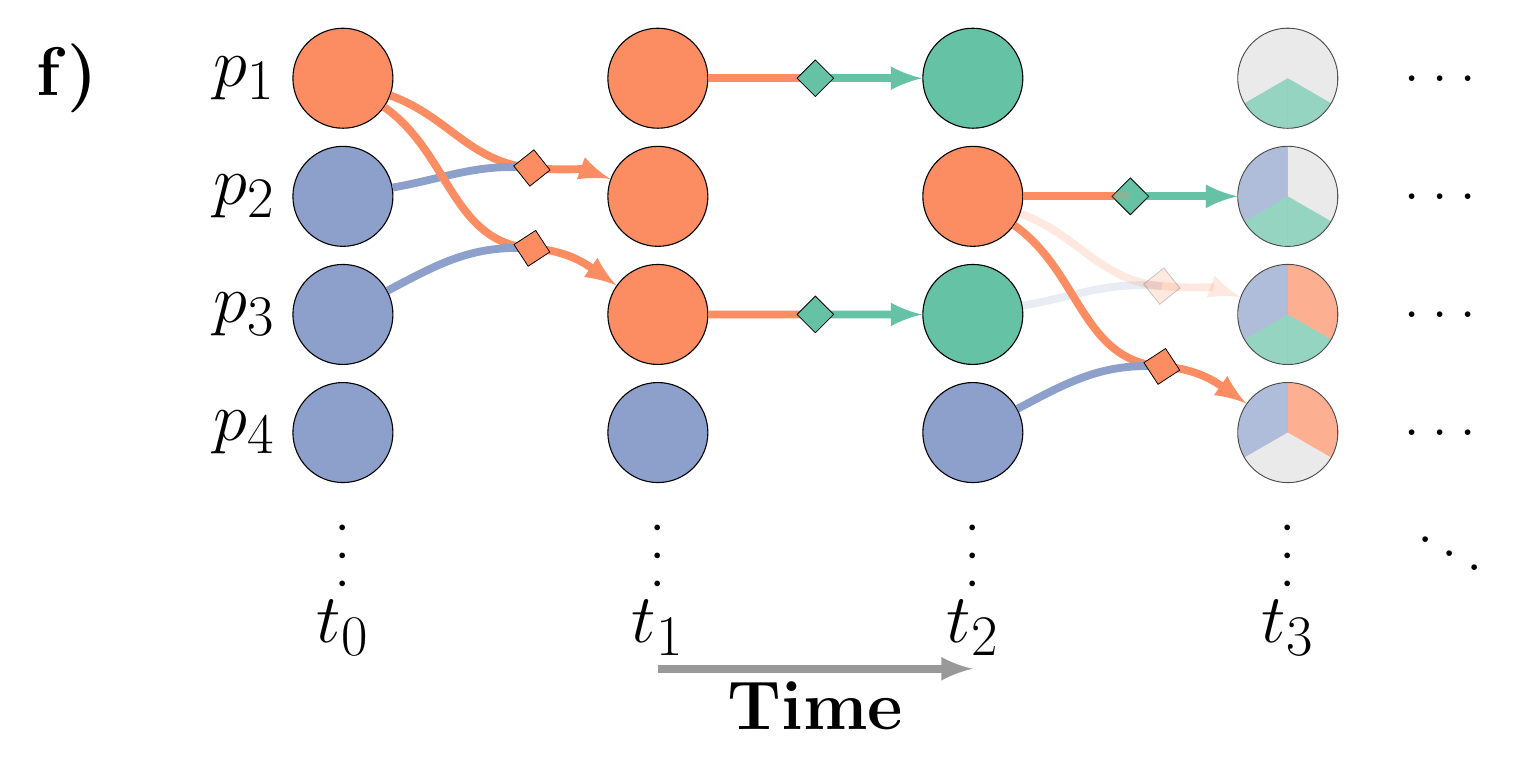
\begin{tikzpicture}
  \draw (-3.5,0) node {\Huge \textbf{f)}};
  \draw (0,0) node[node,actual,circle,fill=infection] (P11) {};
  \draw (0,1.5) node[node,actual,circle,fill=susceptible] (P21) {};
  \draw (0,3) node[node,actual,circle,fill=susceptible] (P31) {};
  \draw (0,4.5) node[node,actual,circle,fill=susceptible] (P41) {};

  \draw (4,0) node[node,actual,circle,fill=infection] (P12) {};
  \draw (4,1.5) node[node,actual,circle,fill=infection] (P22) {};
  \draw (4,3) node[node,actual,circle,fill=infection] (P32) {};
  \draw (4,4.5) node[node,actual,circle,fill=susceptible] (P42) {};

  \draw (8,0) node[node,actual,circle,fill=recovery] (P13) {};
  \draw (8,1.5) node[node,actual,circle,fill=infection] (P23) {};
  \draw (8,3) node[node,actual,circle,fill=recovery] (P33) {};
  \draw (8,4.5) node[node,actual,circle,fill=susceptible] (P43) {};

  \draw (12,0) node[node,potential,circle tri split part fill={nothing,nothing,recovery}] (P14) {};
  \draw (12,1.5) node[node,potential,circle tri split part fill={susceptible,nothing,recovery}] (P24) {};
  \draw (12,3) node[node,potential,circle tri split part fill={susceptible,infection,recovery}] (P34) {};
  \draw (12,4.5) node[node,potential,circle tri split part fill={susceptible,infection,nothing}] (P44) {};

  \contactedge{P11}{P21}{P22}{actual,line width=1mm}{susceptible}{infection}{.6}{10}{-20}
  \contactedge{P11}{P31}{P32}{actual,line width=1mm}{susceptible}{infection}{.7}{28}{-35}
  
  \independentedge{P12}{P13}{actual,line width=1mm}{infection}{recovery};
  \independentedge{P32}{P33}{actual,line width=1mm}{infection}{recovery};
  
  \contactedge{P23}{P33}{P34}{impossible,line width=1mm}{susceptible}{infection}{.6}{10}{-20}
  \contactedge{P23}{P43}{P44}{actual,line width=1mm}{susceptible}{infection}{.7}{28}{-35}
 
  \independentedge{P23}{P24}{actual,line width=1mm}{infection}{recovery};
 
  \independentedge{P23}{P24}{potential,line width=1mm}{infection}{recovery};

  %% Extends on
  \draw (14,0) node{\Huge \dots};
  \draw (14,1.5) node{\Huge \dots};
  \draw (14,3) node{\Huge \dots};
  \draw (14,4.5) node{\Huge \dots};

  \draw (0,6) node[rotate=90]{\Huge \dots};
  \draw (4,6) node[rotate=90]{\Huge \dots};
  \draw (8,6) node[rotate=90]{\Huge \dots};
  \draw (12,6) node[rotate=90]{\Huge \dots};
  \draw (14,6) node[rotate=150]{\Huge \dots};
  %% Legend things
  \draw[-latex,line width=1mm,white!60!black] (4,7.5) -- (8,7.5) node[midway, below,text=black] {\Huge \textbf{Time}};
  \draw (0 ,6.5) node[below,text=black] {\Huge $t_0$};
  \draw (4 ,6.5) node[below,text=black] {\Huge $t_1$};
  \draw (8 ,6.5) node[below,text=black] {\Huge $t_2$};
  \draw (12,6.5) node[below,text=black] {\Huge $t_3$};
  \draw (-1.25,0  ) node[text=black] {\Huge $p_1$};
  \draw (-1.25,1.5) node[text=black] {\Huge $p_2$};
  \draw (-1.25,3  ) node[text=black] {\Huge $p_3$};
  \draw (-1.25,4.5) node[text=black] {\Huge $p_4$};
\end{tikzpicture}

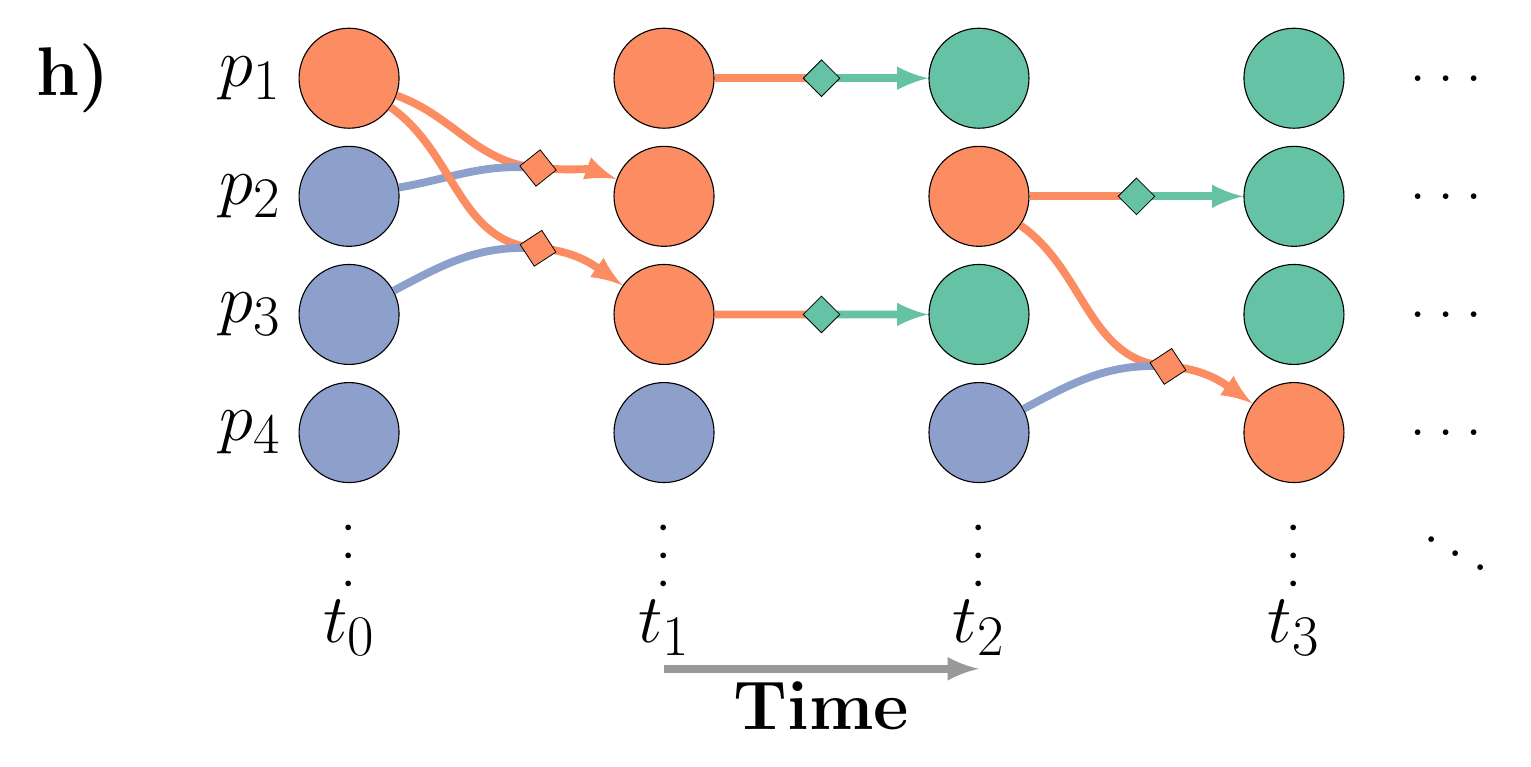
\begin{tikzpicture}
  \draw (-3.5,0) node {\Huge \textbf{h)}};
  \draw (0,0) node[node,actual,circle,fill=infection] (P11) {};
  \draw (0,1.5) node[node,actual,circle,fill=susceptible] (P21) {};
  \draw (0,3) node[node,actual,circle,fill=susceptible] (P31) {};
  \draw (0,4.5) node[node,actual,circle,fill=susceptible] (P41) {};

  \draw (4,0) node[node,actual,circle,fill=infection] (P12) {};
  \draw (4,1.5) node[node,actual,circle,fill=infection] (P22) {};
  \draw (4,3) node[node,actual,circle,fill=infection] (P32) {};
  \draw (4,4.5) node[node,actual,circle,fill=susceptible] (P42) {};

  \draw (8,0) node[node,actual,circle,fill=recovery] (P13) {};
  \draw (8,1.5) node[node,actual,circle,fill=infection] (P23) {};
  \draw (8,3) node[node,actual,circle,fill=recovery] (P33) {};
  \draw (8,4.5) node[node,actual,circle,fill=susceptible] (P43) {};

  \draw (12,0) node[node,actual,circle,fill=recovery] (P14) {};
  \draw (12,1.5) node[node,actual,circle,fill=recovery] (P24) {};
  \draw (12,3) node[node,actual,circle,fill=recovery] (P34) {};
  \draw (12,4.5) node[node,actual,circle,fill=infection] (P44) {};

  \contactedge{P11}{P21}{P22}{actual,line width=1mm}{susceptible}{infection}{.6}{10}{-20}
  \contactedge{P11}{P31}{P32}{actual,line width=1mm}{susceptible}{infection}{.7}{28}{-35}
  
  \independentedge{P12}{P13}{actual,line width=1mm}{infection}{recovery};
  \independentedge{P32}{P33}{actual,line width=1mm}{infection}{recovery};
  
  \contactedge{P23}{P43}{P44}{actual,line width=1mm}{susceptible}{infection}{.7}{28}{-35}
 
  \independentedge{P23}{P24}{actual,line width=1mm}{infection}{recovery};

  %% Extends on
  \draw (14,0) node{\Huge \dots};
  \draw (14,1.5) node{\Huge \dots};
  \draw (14,3) node{\Huge \dots};
  \draw (14,4.5) node{\Huge \dots};

  \draw (0,6) node[rotate=90]{\Huge \dots};
  \draw (4,6) node[rotate=90]{\Huge \dots};
  \draw (8,6) node[rotate=90]{\Huge \dots};
  \draw (12,6) node[rotate=90]{\Huge \dots};
  \draw (14,6) node[rotate=150]{\Huge \dots};
  %% Legend things
  \draw[-latex,line width=1mm,white!60!black] (4,7.5) -- (8,7.5) node[midway, below,text=black] {\Huge \textbf{Time}};
  \draw (0 ,6.5) node[below,text=black] {\Huge $t_0$};
  \draw (4 ,6.5) node[below,text=black] {\Huge $t_1$};
  \draw (8 ,6.5) node[below,text=black] {\Huge $t_2$};
  \draw (12,6.5) node[below,text=black] {\Huge $t_3$};
  \draw (-1.25,0  ) node[text=black] {\Huge $p_1$};
  \draw (-1.25,1.5) node[text=black] {\Huge $p_2$};
  \draw (-1.25,3  ) node[text=black] {\Huge $p_3$};
  \draw (-1.25,4.5) node[text=black] {\Huge $p_4$};
\end{tikzpicture}
\end{document}
